\documentclass{report}

%%%%%%%%%%%%%%%%%%%%%%%%%% Practice info %%%%%%%%%%%%%%%%%%%%%%%%%%
\Subject {Системи штучного інтелекту}
\DocTitle{Обчислення в обчислювальних графах: зворотне поширення помилки}
\ReportType{Семінар}

%----------------------------------------------------
%	  Персональна інформація виконавця завдання
%----------------------------------------------------
\Done{Виконав:}  % Поставте правильне закінчення


\Surname{Бардін}  % Вкажіть своє прізвище
\Name{Владислав}			% та ім'я
\Group {ІМ-42мп}     % група в якій навчаєтесь
\YearOfStudying {5} % курс навчання


%%%%%%%%%%%%%%%%%%%%%%%%%%	 ПОЧАТОК ЗВІТУ	 %%%%%%%%%%%%%%%%%%%%%%%%
\startDocument

\newpage
\section{\doctitle}
	Обчислювальні графи (computational graphs) сьогодні відіграють вирішальну роль у сфері штучного інтелекту та машинного навчання. Саме завдяки обчислювальним графам стає можливим ефективно реалізовувати автоматичне диференціювання та розуміти, як зміна окремих параметрів впливає на кінцевий результат. Алгоритм зворотного поширення помилки (backpropagation) — один із найважливіших інструментів оптимізації параметрів у нейронних мережах, що дав змогу перейти від теоретичного концепту багатошарових мереж до їх успішного практичного застосування.
Актуальність теми визначається тим, що зворотне поширення помилки продовжує залишатися основою більшості сучасних підходів до навчання глибинних моделей, у тому числі таких, що використовуються в розпізнаванні образів, обробці природної мови та побудові рекомендаційних систем. Тому розуміння механізму розрахунків у обчислювальних графах, а також принципів та особливостей backpropagation є необхідною складовою підготовки кваліфікованих фахівців у галузі комп’ютерних наук.
Мета даного реферату полягає у комплексному аналізі технології обчислень в обчислювальних графах та детальному розгляді алгоритму зворотного поширення помилки. Для досягнення поставленої мети виділено такі завдання:
\begin{itemize}
	\item	розглянути базові поняття та історію виникнення обчислювальних графів;
	\item проаналізувати ключові принципи зворотного поширення помилки та описати його математичне підґрунтя;
	\item дослідити застосування зворотного поширення у навчанні нейронних мереж, виявити типові труднощі і шляхи їх подолання.
\end{itemize}
У процесі дослідження в рефераті будуть використані теоретичні методи (аналіз літератури та існуючих підходів), а також огляд практичних прикладів із різних галузей. У підсумку, це дасть змогу скласти цілісне уявлення про суть та перспективи технології зворотного поширення помилки, її значення для подальшого розвитку систем штучного інтелекту.

\newpage
\section{Поняття обчислювальних графів}
Обчислювальний граф (computational graph) — це математична модель, у якій обчислювальний процес представлений у вигляді орієнтованого графа. Вузли (вершини) такого графа відповідають операціям або функціям, що виконуються над даними (наприклад, додавання, множення, застосування активаційної функції тощо), а ребра (дуги) відображають передачу результатів цих операцій від одного вузла до іншого.
Ключовою особливістю обчислювального графа є поділ обчислень на послідовні кроки, де кожен вузол виконує конкретну операцію, спираючись на вхідні дані, отримані з попередніх вузлів. Така структура надає можливість:
\begin{itemize}
	\item наглядно відстежувати весь ланцюг обчислень;
	\item автоматизувати процес диференціювання;
	\item ефективно розподіляти обчислення.
\end{itemize}
Завдяки цьому можна легко проаналізувати, яким чином початкові вхідні змінні впливають на кінцевий результат, а також кроки, що не залежать один від одного, можуть виконуватися паралельно, що робить обчислення швидшими та ефективнішими.
У сучасних фреймворках (наприклад, TensorFlow чи PyTorch) побудований обчислювальний граф дозволяє задіяти вбудовані механізми автоматичного обчислення градієнтів; це спрощує та прискорює процес навчання нейронних мереж.
Як приклад розглянемо просту функцію з двома змінними x та y:
\begin{equation}
	f(x,y)=(x+y)  ×y
\end{equation}

\begin{figure}[hbt!]
  \center
  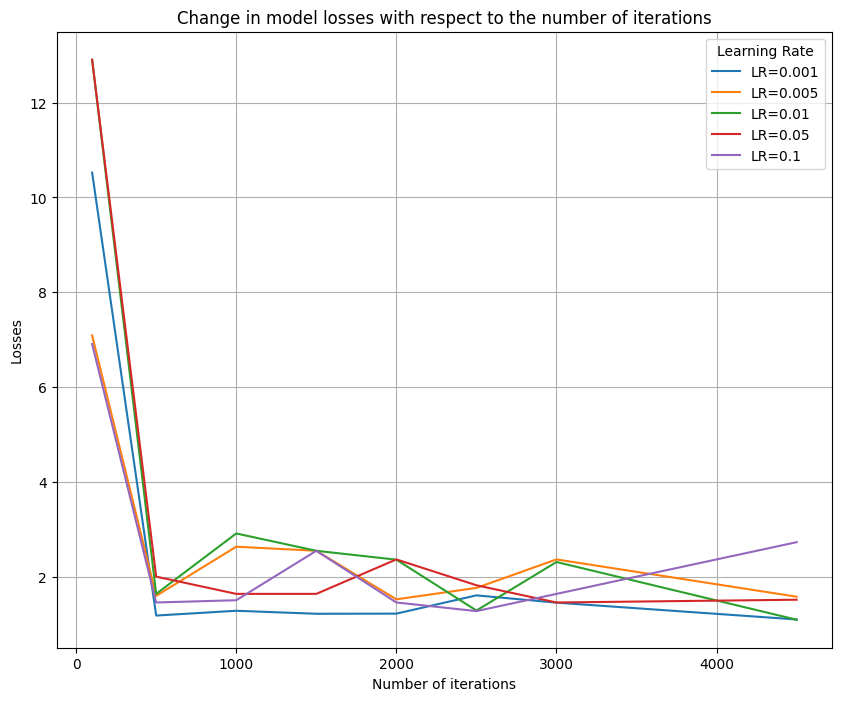
\includegraphics[scale=0.5]{fig1}
  \caption{Обчислювальний граф для функції}
   \label{im:fig1}
\end{figure}
Обчислення цього графу можна подати у вигляді вузла А, який отримує 2 вхідні параметри x та y, та виконує операцію додавання x+y. Та вузла Б, який отримує як вхідні параметри y та результат виконання вузла А (x+y) виконуючи множення ((x+y)×y).
Сформувавши таку схему нею можна зробити 2 проходи, у прямому (forward pass) та зворотному напрямку (backward pass). Прямий обхід застосовується для обчислення кінцевого значення функції, а зворотній для обчислення градієнтів відносно змінних x та y.

Завдяки такому підходу у складних нейронних мережах з багатьма шарами і безліччю параметрів ми можемо системно структурувати процес. Замість монолітного обчислення маємо послідовну (або й паралельну) сукупність вузлів і ребер, де кожна операція виконується у чітко визначеному порядку.
Таким чином, обчислювальні графи є фундаментом для реалізації алгоритму зворотного поширення помилки, оскільки саме завдяки чіткій структурі вузлів і ребер можна коректно та швидко знайти градієнти кожного параметра, впливаючи на точність і швидкість навчання штучних нейронних мереж.

\newpage
\section{Загальна ідея алгоритму зворотного поширення помилки}

Зворотне поширення помилки (англ. backpropagation) — це алгоритм, який дозволяє “навчити” штучну нейронну мережу коригувати свої внутрішні параметри з метою мінімізувати функцію помилки (англ. error function). Його ефективність ґрунтується на застосуванні правила ланцюгового диференціювання, що дає змогу обчислити, як саме зміна кожного параметра впливає на кінцеву похибку мережі.

Ідеї зворотного поширення помилки були сформульовані в роботах Джефрі Гінтона, Девіда Румельхарта та Рональда Вільямса ще у 1980-х роках. Саме цей алгоритм зробив можливим успішне навчання багатошарових нейронних мереж, які до того вважалися непрактичними для реальних задач.

Усі обчислення можна представити в вигляді обчислювального графа: кожен шар є вузлом, ребра відображають передачу результатів між шарами. Зворотний прохід природно відповідає “руху” цим графом у зворотному напрямі, дозволяючи підрахувати необхідні похідні автоматично.
Для виконання прямого проходу вхідні дані подаються на вхід мережі, проходять через усі шари з відповідними функціями активації, і на виході отримується прогноз. Після цього обчислюється значення функції помилки, наприклад, сума квадратів різниць між передбаченими та реальними виходами, або крос-ентропія. Обчислене значення функції помилки використовується для руху у зворотному напрямку, послідовно обчислюючи частинні похідні відносно кожної ваги. Таким чином ми отримуємо інформацію про те, як змінити кожен параметр мережі, щоб зменшити загальну помилку.

У загальному випадку, якщо вихідна помилка позначається як E, а проміжна змінна як z, то похідну dE/dz можна обчислити через інші змінні u,v… згідно з правилом ланцюга:
\begin{equation}
	\frac{dE}{dz} = \frac{dE}{du} \cdot \frac{du}{dv} \cdot \dots \cdot \frac{dw}{dz}
\end{equation}
У контексті нейронної мережі кожен “ланцюг” відповідає шляху в обчислювальному графі від параметра до підсумкової функції помилки.
Після обчислення градієнтів алгоритм зворотного поширення помилки зазвичай застосовується у поєднанні з методом градієнтного спуску, який оновлює кожну вагу $W_{ij}$ у напрямку протилежному до градієнта:
\begin{equation}
	W_{ij} \leftarrow W_{ij} - \eta \cdot \frac{dE}{dW_{ij}}
\end{equation}

де $\eta$ – швидкість навчання.
 
Це дозволяє послідовно зменшувати значення функції помилки на кожній ітерації, поки мережа не досягне прийнятної точності.

Загалом, алгоритм зворотного поширення помилки — це “серце” навчання більшості глибинних нейронних мереж. Він дає змогу поєднати переваги обчислювальних 
графів з математикою ланцюгового диференціювання, що в підсумку забезпечує ефективне й точне оновлення параметрів моделі.

\newpage
\section{ВИСНОВКИ}

Зворотне поширення помилки (backpropagation) є фундаментальним алгоритмом, який забезпечив прорив у сфері машинного навчання та глибинних нейронних мереж. Завдяки послідовному обчисленню градієнтів кожного параметра мережі та врахуванню усіх проміжних операцій в обчислювальному графі стало можливим навчати багатошарові моделі та отримувати вражаючі результати в різноманітних завданнях: від комп’ютерного зору до обробки природної мови і рекомендаційних систем.
У ході роботи над рефератом проаналізовано:
\begin{itemize}
	\item суть обчислювальних графів: їхня роль у структуризації всього процесу обчислень та наочне представлення операцій над даними;
	\item механізм та ідея backpropagation: від історичних витоків до конкретного алгоритмічного втілення; описано, як кожен параметр впливає на помилку на виході і як його оновити за правилом ланцюгового диференціювання.
\end{itemize}

Застосування зворотного поширення помилки разом із потужними засобами апаратного прискорення дає змогу обробляти величезні обсяги даних, будувати глибинні мережі й успішно розв’язувати складні прикладні завдання. Попри наявність альтернативних підходів, backpropagation залишається основою більшості сучасних рішень у галузі штучного інтелекту.

Backpropagation має перспективи подальших досліджень, що полягають у розробці покращених методів оптимізації, вивченні способів розв’язання проблеми зникаючих та вибухаючих градієнтів, а також у пошуку нових архітектур, здатних ще ефективніше використовувати потенціал зворотного поширення помилки. Це означає, що backpropagation та обчислювальні графи залишатимуться важливою складовою інструментарію машинного навчання у найближчому майбутньому.

\newpage

\begin{thebibliography}{99}

\bibitem{Goodfellow2016}
Goodfellow, I., Bengio, Y., and Courville, A. \textit{Deep Learning}. MIT Press, 2016.

\bibitem{Rumelhart1986}
Rumelhart, D. E., Hinton, G. E., and Williams, R. J. Learning representations by back-propagating errors. \textit{Nature}, 1986, Vol. 323, pp. 533-536.

\bibitem{Werbos1982}
Werbos, P. J. Applications of advances in nonlinear sensitivity analysis. \textit{System Modeling and Optimization}, Springer, Berlin, Heidelberg, 1982, pp. 762-770.

\bibitem{Nielsen2015}
Nielsen, M. \textit{Neural Networks and Deep Learning}. 2015. Retrieved from \url{http://neuralnetworksanddeeplearning.com}.

\bibitem{Bishop2006}
Bishop, C. M. \textit{Pattern Recognition and Machine Learning}. Springer, 2006.

\end{thebibliography}
\end{document}
